


\chapter*{Implementation - Architecture}
\addcontentsline{toc}{chapter}{Architecture}

  In case you haven't read the previous chapter i advise glimsing over the chapters' titles at least once because it would give better context on where my project lives in the graphics lifecycle.

  My Application is a Graphics Abstraction Layer that imitates industry standards when it comes to procedures used for ease of learning.
  Besides being an easy-to-use beginner-friendly tool because of following industry standard solution in the c++ rendering backend engine. At it's core, this rendering engine is built on top of a vectorial mathematics engine.

  The novelty that this project brings to the computer graphics world is the presence of a python Machine Learning backend that acts as an abstraction layer for simplifying the communication with services (openai, ollama) or with powerful machine learning libraries (scipy, skilearn) 
  
  \begin{figure}
    \begin{center}
      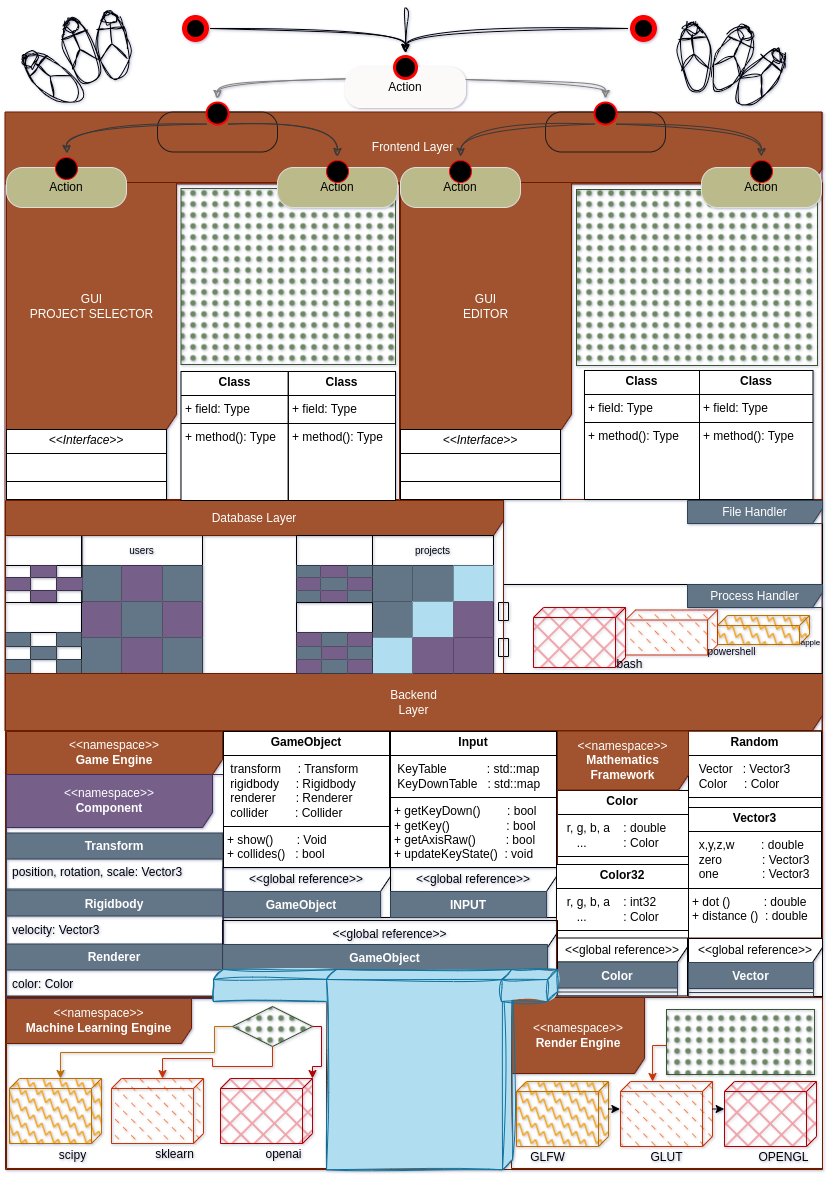
\includegraphics[width=\textwidth]{implementation_arch.png}
    \caption{Arch}
    \end{center}
  \end{figure}
  \pagebreak


  \section*{The backend}
    The Backend is wrote mostly in C++ and offers the user namespaces to interact with the opengl inner-workings of the engine.

    \begin{figure}
      \begin{center}
        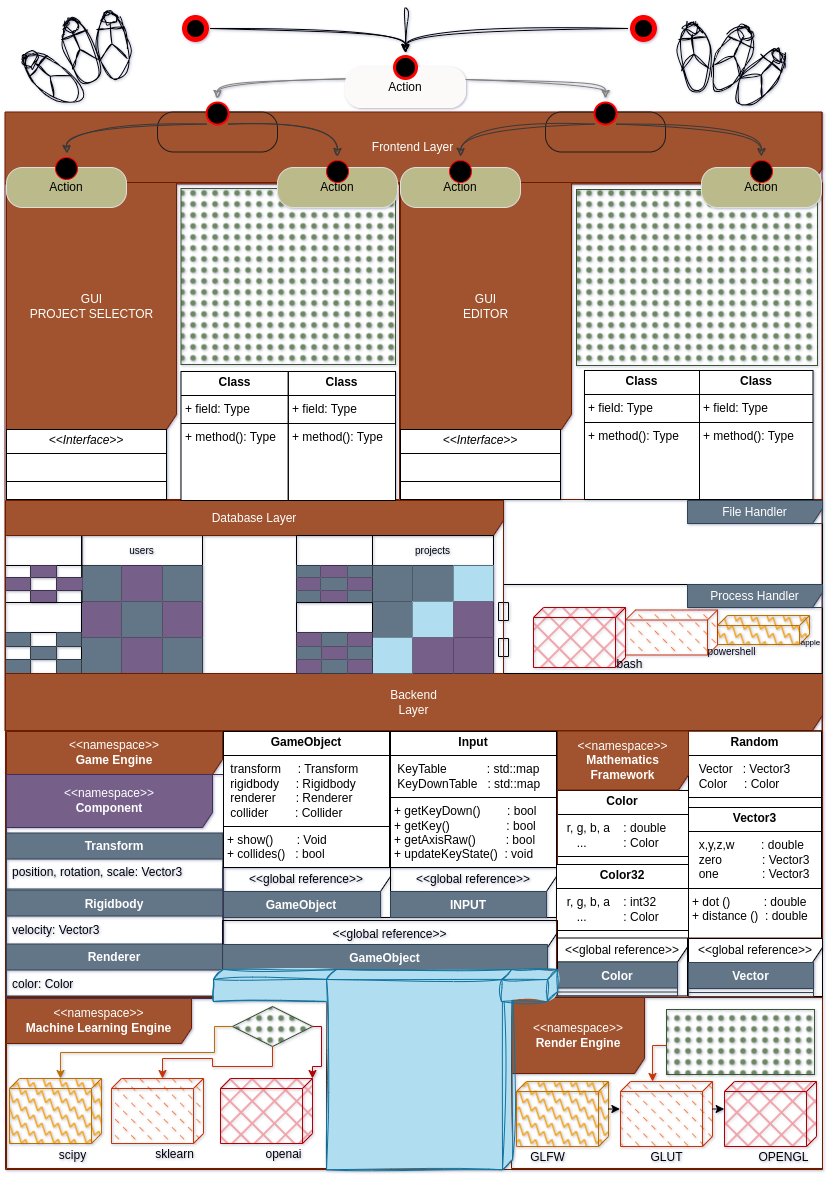
\includegraphics[width=\textwidth]{implementation_arch.png}
      \caption{Arch}
      \end{center}
    \end{figure}
    \pagebreak

  \section*{The Frontend}

    The frontend is wrote mostly in Python with the help of PyQt, a python wrapper for the industry standard qt.

    \begin{figure}
      \begin{center}
        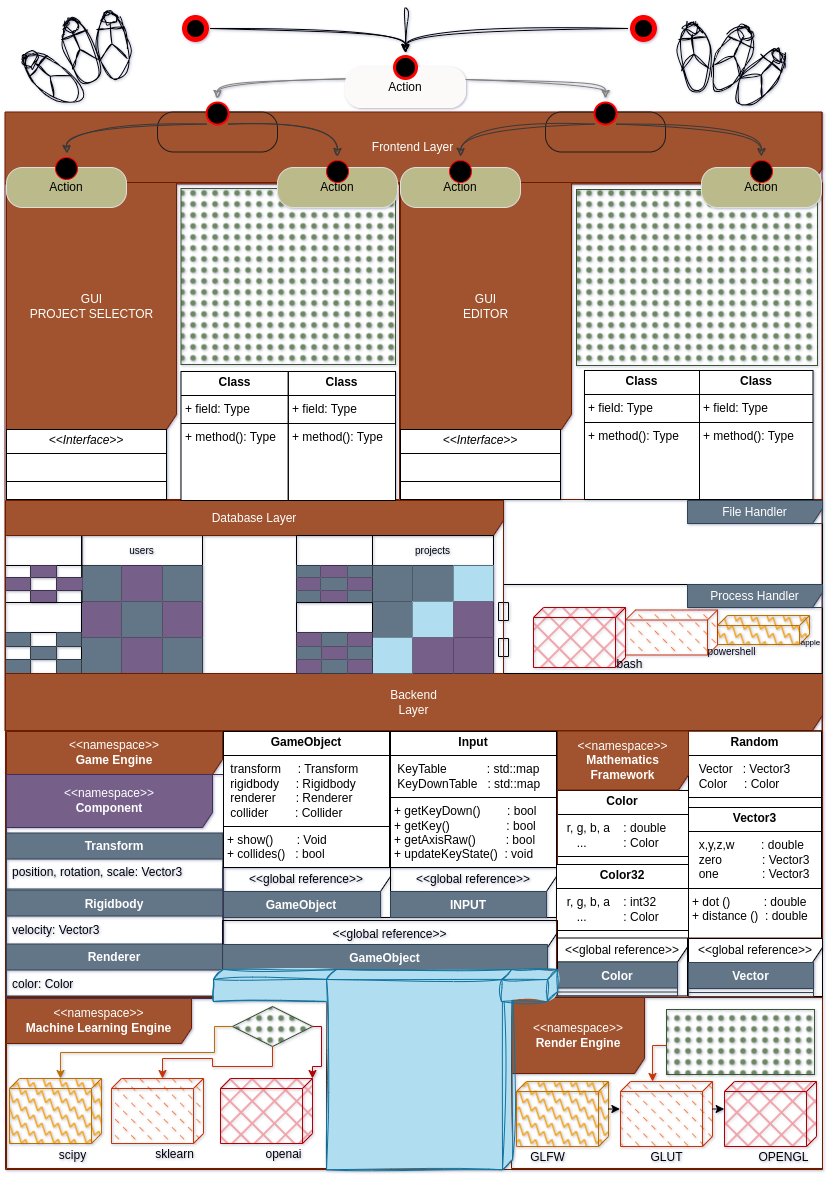
\includegraphics[width=\textwidth]{implementation_arch.png}
      \caption{Arch}
      \end{center}
    \end{figure}
    \pagebreak

  \section*{Additional Tools}

    Additional tools has been developed already, tools that improves the programmer's workflow.
    Such example is a web scraper for data collecting.
    Docs for each major component.
    \begin{figure}
      \begin{center}
        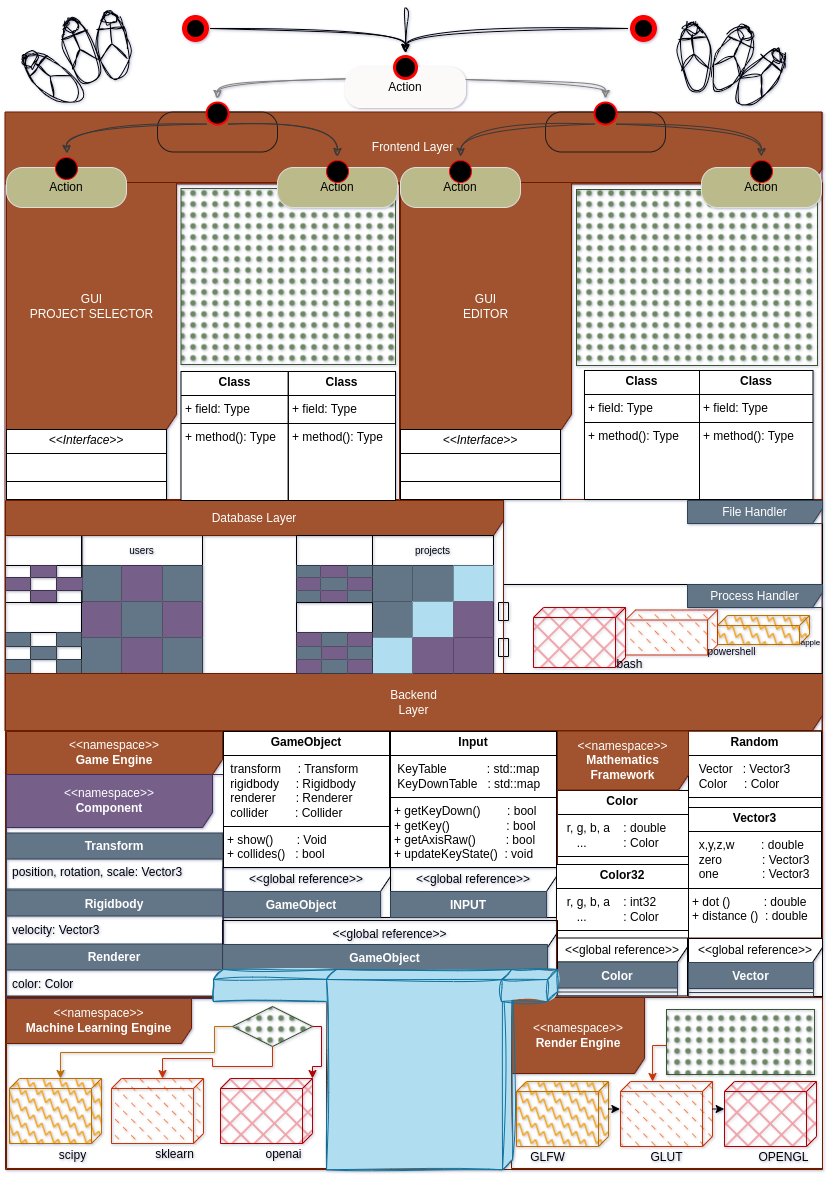
\includegraphics[width=\textwidth]{implementation_arch.png}
      \caption{Arch}
      \end{center}
    \end{figure}
    \pagebreak
